\documentclass[residuals.tex]{subfiles}
\begin{document}
\Large
\section{Outliers and Influential Observations}
\begin{quote}
	``Outliers are sample values that cause surprise in relation to the majority of the sample" (W.N. Venables and B.D. Ripley. 2002. Modern applied statistics with S. New York: Springer, p.119).
\end{quote}
\begin{itemize}
\item Crucially, surprise is in the mind of the beholder and is dependent on some explicit model of the data. 

\item Importantly, Normality is only an assumption : There may be another model under which the outlier is not surprising at all, say if the data really are lognormal or 
gamma rather than normally distributed. 
\end{itemize}

\subsection{Regression Outliers}

Data points that diverge in a big way from the overall pattern are referred to as ``outliers".
In the case of Simple Linear Regression, there are four ways that a data point might be considered an outlier.
%---------------------------------------------------------%
\begin{framed}
\begin{itemize}
	\item It could have an extreme X value compared to other data points.
	\item It could have an extreme Y value compared to other data points.
	\item It could have extreme X and Y values.
	\item It might be distant from the rest of the data, even without extreme X or Y values.
\end{itemize}
\end{framed}
\begin{figure}[h!]
\centering
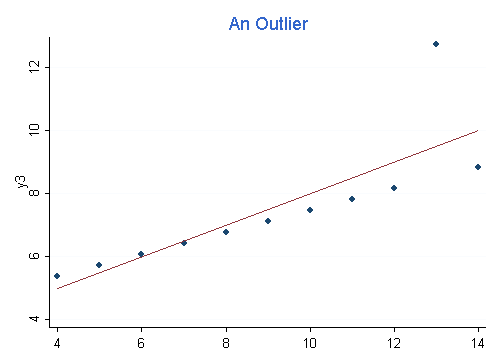
\includegraphics[width=0.7\linewidth]{regressionoutlier}
\end{figure}

%---------------------------------------------------------%
\begin{itemize}
\item After a regression line has been computed for a group of data, a point which lies far from the line 
(and thus has a large residual value) is known as an outlier. 
Such points may represent erroneous data, or may indicate a poorly fitting regression line. 

\item If a point lies far from the other data in the horizontal direction, it is known as an \textit{\textbf{influential observation}}. 
The reason for this distinction is that these points have may have a significant impact on the slope of the regression line.
\end{itemize}

\Large
\section*{Testing for Regression Outliers with \texttt{R}}
\begin{itemize}
\item Suppose we have  two unseen fitted models and we would like to see if there are any outliers. 

\item For this purpose, we can use \texttt{outlierTest()} from \texttt{library(car)} in \texttt{R}.
\item In the first example, two outliers are detected.
\item For the second fitted model, no outliers are detected. The most unusual observation, relative to the rest of the data set, is reported instead.
\end{itemize}
 

%Currently facing a problem in interpreting the results.


\begin{framed}
	\begin{verbatim}
	library(car)
	outlierTest(fit1)   
	
	**Result:**
	   rstudent unadjusted p-value  Bonferonni p
	21    -4.12            4.39e-05        0.0209
	15    -4.08            5.39e-05        0.0257
	
	outlierTest(fit2)   
	
	**Result:**
	No Studentized residuals with Bonferonni p < 0.05
	Largest |rstudent|:
  	    rstudent unadjusted p-value      Bonferonni p
	177    -2.52             0.0119                NA
	\end{verbatim}
\end{framed}

The row numbers (here : 21, 15) indicate the outlier points in the first fitted model. Case 177 is the most unusual case from the second model, but not an outlier.


\end{document}
